\documentclass{standalone}
\usepackage{tikz}
\usetikzlibrary{patterns, positioning}
\usepackage[sfdefault]{ClearSans} %% option 'sfdefault' activates Clear Sans as the default text font
\usepackage[T1]{fontenc}

\begin{document}
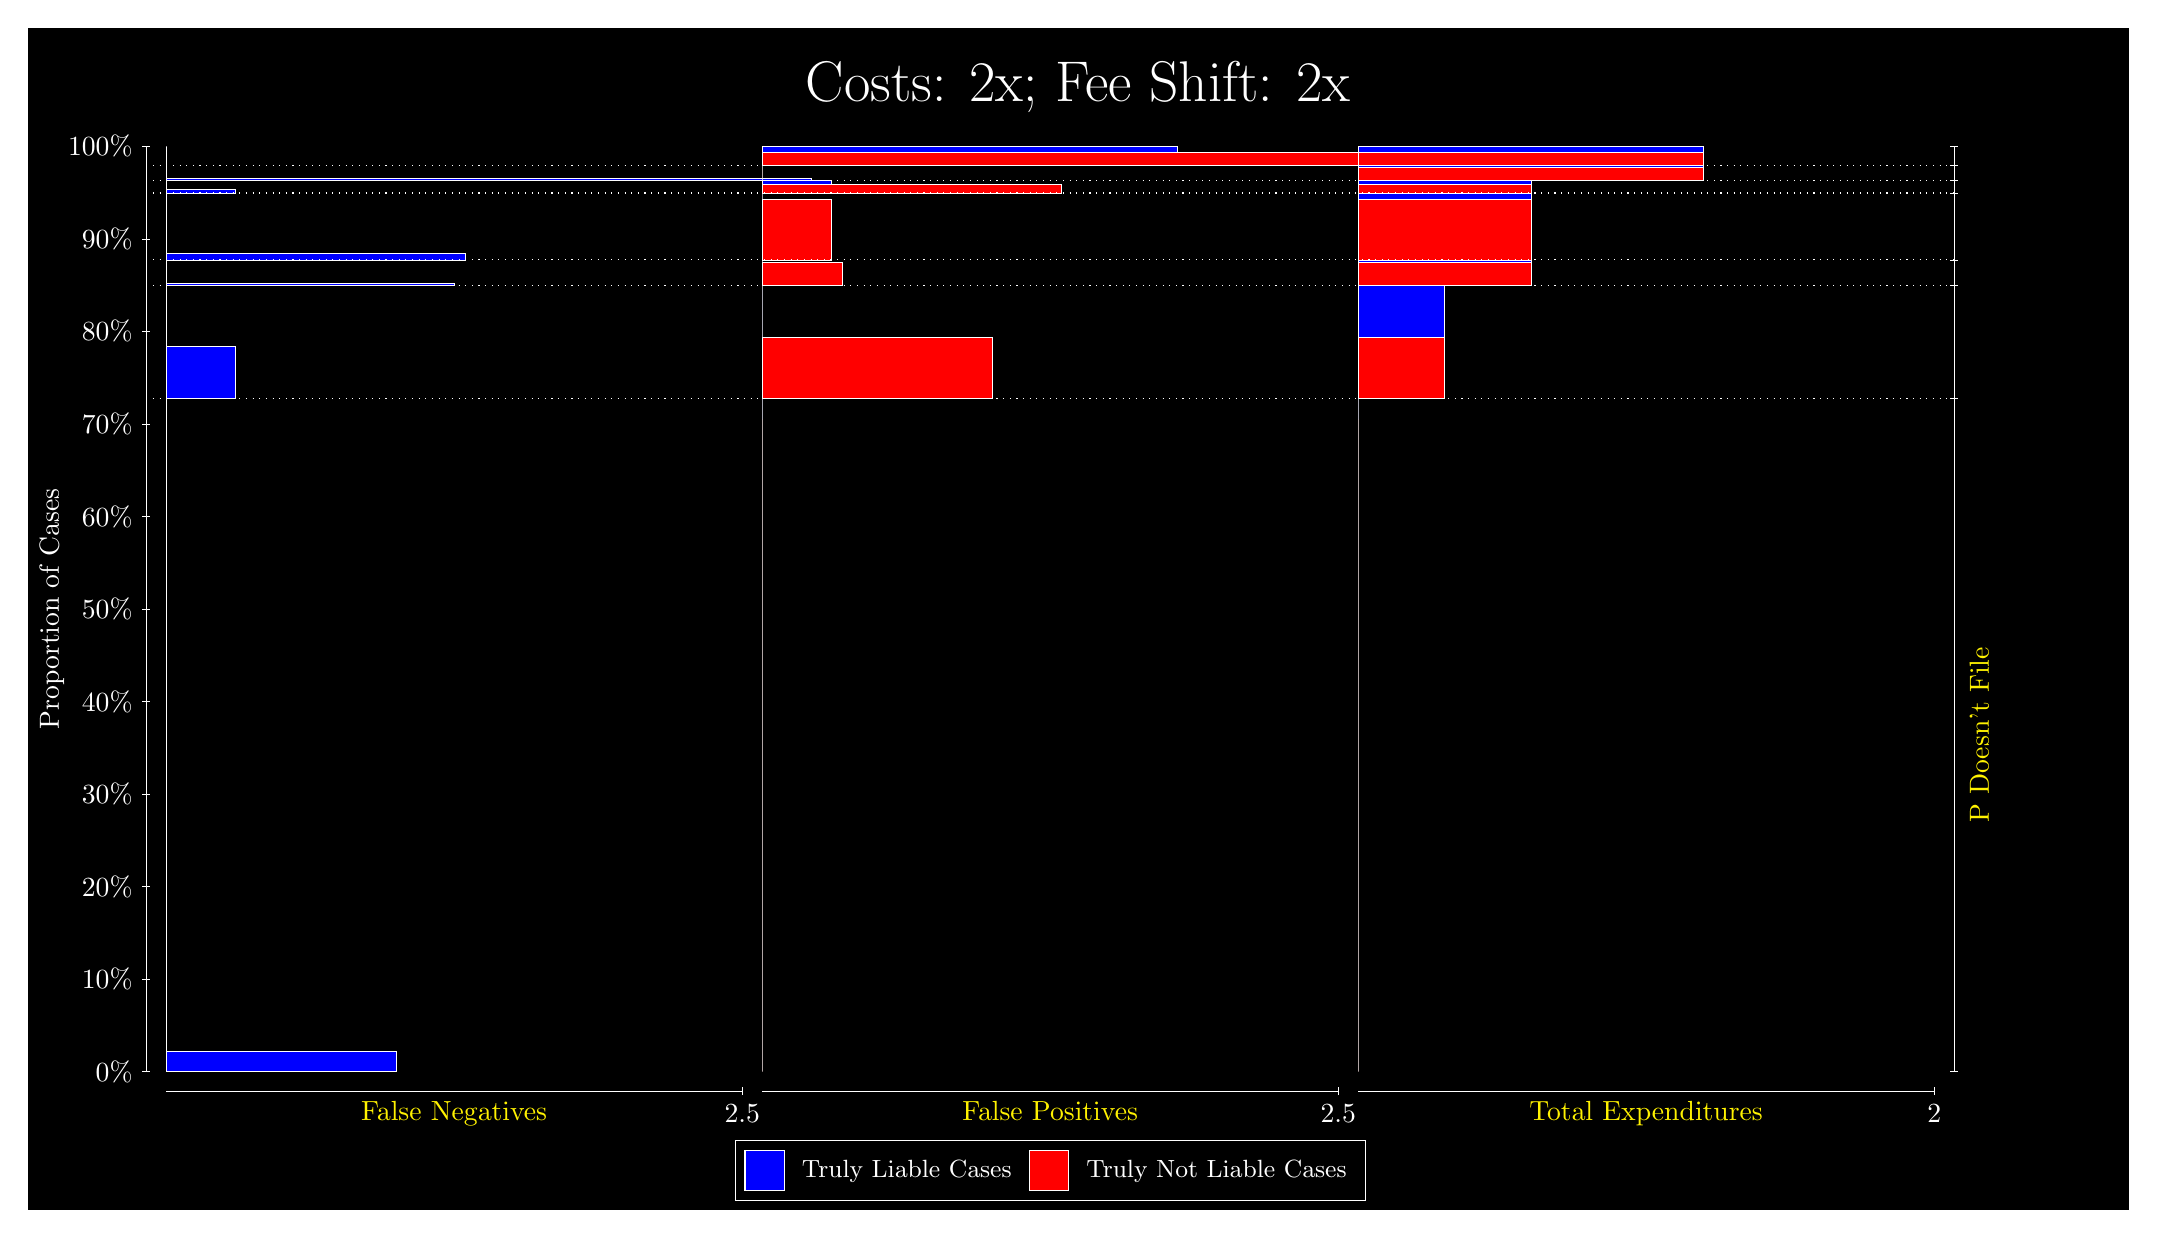
\begin{tikzpicture}
\draw[fill=black] (0,0) rectangle (26.667,15);
\draw[text=white] (0,13.5) rectangle (26.667,15) node[midway] {\huge Costs: 2x; Fee Shift: 2x};
\draw[white, very thin] (1.5,1.75) -- (1.5,13.5);
\node[rotate=90, text=white, anchor=center] at (0.3, 7.625) {Proportion of Cases};
\draw[white, very thin] (1.45,1.75) -- (1.55,1.75);
\node[text=white, anchor=east] at (1.45, 1.75) {0\%};
\draw[white, very thin] (1.45,2.925) -- (1.55,2.925);
\node[text=white, anchor=east] at (1.45, 2.925) {10\%};
\draw[white, very thin] (1.45,4.1) -- (1.55,4.1);
\node[text=white, anchor=east] at (1.45, 4.1) {20\%};
\draw[white, very thin] (1.45,5.275) -- (1.55,5.275);
\node[text=white, anchor=east] at (1.45, 5.275) {30\%};
\draw[white, very thin] (1.45,6.45) -- (1.55,6.45);
\node[text=white, anchor=east] at (1.45, 6.45) {40\%};
\draw[white, very thin] (1.45,7.625) -- (1.55,7.625);
\node[text=white, anchor=east] at (1.45, 7.625) {50\%};
\draw[white, very thin] (1.45,8.8) -- (1.55,8.8);
\node[text=white, anchor=east] at (1.45, 8.8) {60\%};
\draw[white, very thin] (1.45,9.975) -- (1.55,9.975);
\node[text=white, anchor=east] at (1.45, 9.975) {70\%};
\draw[white, very thin] (1.45,11.15) -- (1.55,11.15);
\node[text=white, anchor=east] at (1.45, 11.15) {80\%};
\draw[white, very thin] (1.45,12.325) -- (1.55,12.325);
\node[text=white, anchor=east] at (1.45, 12.325) {90\%};
\draw[white, very thin] (1.45,13.5) -- (1.55,13.5);
\node[text=white, anchor=east] at (1.45, 13.5) {100\%};

\draw[white, very thin] (24.457,1.75) -- (24.457,13.5);
\draw[white, very thin] (24.407,1.75) -- (24.507,1.75);
\node[anchor=west] at (24.407, 1.75) {};
\draw[white, very thin] (24.407,10.297) -- (24.507,10.297);
\node[anchor=west] at (24.407, 10.297) {};
\draw[white, very thin] (24.407,11.737) -- (24.507,11.737);
\node[anchor=west] at (24.407, 11.737) {};
\draw[white, very thin] (24.407,12.058) -- (24.507,12.058);
\node[anchor=west] at (24.407, 12.058) {};
\draw[white, very thin] (24.407,12.907) -- (24.507,12.907);
\node[anchor=west] at (24.407, 12.907) {};
\draw[white, very thin] (24.407,13.07) -- (24.507,13.07);
\node[anchor=west] at (24.407, 13.07) {};
\draw[white, very thin] (24.407,13.254) -- (24.507,13.254);
\node[anchor=west] at (24.407, 13.254) {};
\draw[white, very thin] (24.407,13.5) -- (24.507,13.5);
\node[anchor=west] at (24.407, 13.5) {};

\draw[white, very thin, fill=blue] (1.75,1.75) rectangle (4.6775,2.0111);
\draw[white, very thin, fill=red] (1.75,2.0111) rectangle (1.75,10.297);
\draw[white, very thin, fill=blue] (1.75,10.297) rectangle (2.6283,10.96);
\draw[white, very thin, fill=red] (1.75,10.96) rectangle (1.75,11.737);
\draw[white, very thin, fill=blue] (1.75,11.737) rectangle (5.4094,11.762);
\draw[white, very thin, fill=red] (1.75,11.762) rectangle (1.75,12.058);
\draw[white, very thin, fill=blue] (1.75,12.058) rectangle (5.5558,12.141);
\draw[white, very thin, fill=red] (1.75,12.141) rectangle (1.75,12.907);
\draw[white, very thin, fill=blue] (1.75,12.907) rectangle (2.6283,12.956);
\draw[white, very thin, fill=red] (1.75,12.956) rectangle (1.75,13.07);
\draw[white, very thin, fill=blue] (1.75,13.07) rectangle (9.9471,13.089);
\draw[white, very thin, fill=red] (1.75,13.089) rectangle (1.75,13.254);
\draw[white, very thin, fill=red] (1.75,13.254) rectangle (1.75,13.426);
\draw[white, very thin, fill=blue] (1.75,13.426) rectangle (1.75,13.5);
\draw[white, very thin, fill=red] (9.3189,1.75) rectangle (9.3189,10.036);
\draw[white, very thin, fill=blue] (9.3189,10.036) rectangle (9.3189,10.297);
\draw[white, very thin, fill=red] (9.3189,10.297) rectangle (12.246,11.074);
\draw[white, very thin, fill=blue] (9.3189,11.074) rectangle (9.3189,11.737);
\draw[white, very thin, fill=red] (9.3189,11.737) rectangle (10.344,12.033);
\draw[white, very thin, fill=blue] (9.3189,12.033) rectangle (9.3189,12.058);
\draw[white, very thin, fill=red] (9.3189,12.058) rectangle (10.197,12.823);
\draw[white, very thin, fill=blue] (9.3189,12.823) rectangle (9.3189,12.907);
\draw[white, very thin, fill=red] (9.3189,12.907) rectangle (13.125,13.02);
\draw[white, very thin, fill=blue] (9.3189,13.02) rectangle (10.197,13.07);
\draw[white, very thin, fill=red] (9.3189,13.07) rectangle (9.3189,13.235);
\draw[white, very thin, fill=blue] (9.3189,13.235) rectangle (9.3189,13.254);
\draw[white, very thin, fill=red] (9.3189,13.254) rectangle (17.516,13.426);
\draw[white, very thin, fill=blue] (9.3189,13.426) rectangle (14.588,13.5);
\draw[white, very thin, fill=red] (16.888,1.75) rectangle (16.888,10.036);
\draw[white, very thin, fill=blue] (16.888,10.036) rectangle (16.888,10.297);
\draw[white, very thin, fill=red] (16.888,10.297) rectangle (17.986,11.074);
\draw[white, very thin, fill=blue] (16.888,11.074) rectangle (17.986,11.737);
\draw[white, very thin, fill=red] (16.888,11.737) rectangle (19.083,12.033);
\draw[white, very thin, fill=blue] (16.888,12.033) rectangle (19.083,12.058);
\draw[white, very thin, fill=red] (16.888,12.058) rectangle (19.083,12.823);
\draw[white, very thin, fill=blue] (16.888,12.823) rectangle (19.083,12.907);
\draw[white, very thin, fill=red] (16.888,12.907) rectangle (19.083,13.02);
\draw[white, very thin, fill=blue] (16.888,13.02) rectangle (19.083,13.07);
\draw[white, very thin, fill=red] (16.888,13.07) rectangle (21.279,13.235);
\draw[white, very thin, fill=blue] (16.888,13.235) rectangle (21.279,13.254);
\draw[white, very thin, fill=red] (16.888,13.254) rectangle (21.279,13.426);
\draw[white, very thin, fill=blue] (16.888,13.426) rectangle (21.279,13.5);
\draw[white, dotted] (1.5,10.297) -- (24.457,10.297);
\draw[white, dotted] (1.5,11.737) -- (24.457,11.737);
\draw[white, dotted] (1.5,12.058) -- (24.457,12.058);
\draw[white, dotted] (1.5,12.907) -- (24.457,12.907);
\draw[white, dotted] (1.5,13.07) -- (24.457,13.07);
\draw[white, dotted] (1.5,13.254) -- (24.457,13.254);
\draw[white, very thin] (1.75,1.5) -- (9.0689,1.5);
\node[text=yellow, anchor=north] at (5.4094, 1.5) {False Negatives};
\draw[white, very thin] (9.0689,1.45) -- (9.0689,1.55);
\node[text=white, anchor=north] at (9.0689, 1.45) {2.5};

\draw[white, very thin] (9.3189,1.5) -- (16.638,1.5);
\node[text=yellow, anchor=north] at (12.978, 1.5) {False Positives};
\draw[white, very thin] (16.638,1.45) -- (16.638,1.55);
\node[text=white, anchor=north] at (16.638, 1.45) {2.5};

\draw[white, very thin] (16.888,1.5) -- (24.207,1.5);
\node[text=yellow, anchor=north] at (20.547, 1.5) {Total Expenditures};
\draw[white, very thin] (24.207,1.45) -- (24.207,1.55);
\node[text=white, anchor=north] at (24.207, 1.45) {2};

\node[text=yellow, centered, rotate=90] at (24.777, 6.0236) {P Doesn't File};







\draw (12.978300999999998,1.5) node[draw=none] (baseCoordinate) {};
\begin{scope}[align=center]
        \matrix[scale=0.5, draw=white, below=0.5cm of baseCoordinate, nodes={draw}, column sep=0.1cm]{
            \node[rectangle, draw, minimum width=0.5cm, minimum height=0.5cm, fill=blue] {}; &
            \node[draw=none, font=\small, text=white] (B) {Truly Liable Cases}; &
            \node[rectangle, draw, minimum width=0.5cm, minimum height=0.5cm, fill=red] {}; &
            \node[draw=none, font=\small, text=white] (B) {Truly Not Liable Cases}; \\
            };
\end{scope}

\end{tikzpicture}
\end{document}